\documentclass[final]{cvpr}

% NOTE(brendan):
% https://tex.stackexchange.com/questions/398223/tikz-gives-error-command-everyshipouthook-already-defined/398269
\makeatletter
\@namedef{ver@everyshi.sty}{}
\makeatother
\usepackage{tikz}
\usepackage{times}
\usepackage{epsfig}
\usepackage{graphicx}
\usepackage{amsmath}
\usepackage{amssymb}

% Include other packages here, before hyperref.
\usepackage[normalem]{ulem}
\usepackage{siunitx}

% NOTE(brendan): my packages
\usepackage{bbm}  % for \mathbbm{1}
\usepackage{bm}  % for more powerful bold symbols https://tex.stackexchange.com/a/596
\usepackage{caption}
\captionsetup[table]{skip=5pt}  % space between table and caption https://tex.stackexchange.com/a/2836
\usepackage{booktabs}
\usepackage{pifont}  % for dingbats checkmark and xmark

% If you comment hyperref and then uncomment it, you should delete
% egpaper.aux before re-running latex.  (Or just hit 'q' on the first latex
% run, let it finish, and you should be clear).
\usepackage[pagebackref=true,breaklinks=true,letterpaper=true,colorlinks,bookmarks=false]{hyperref}

% NOTE(brendan): my macros
% https://tex.stackexchange.com/a/217624
\makeatletter
\newcommand*{\transpose}{%
	{\mathpalette\@transpose{}}%
}
\newcommand*{\@transpose}[2]{%
	% #1: math style
	% #2: unused
	\raisebox{\depth}{$\m@th#1\intercal$}%
}
\makeatother
\DeclareMathOperator*{\argmax}{arg\,max}
\DeclareMathOperator*{\argmin}{arg\,min}

% \makeatletter                  % You do not need to write [htpb] all the time
% \renewcommand\fps@figure{htbp} %
% \renewcommand\fps@table{htbp}  %
% \makeatother                   %

\def\cvprPaperID{3473} % *** Enter the CVPR Paper ID here
\def\confYear{CVPR 2021}

\newcommand{\myparagraph}[1]{\textbf{#1 ---}}


\begin{document}

\title{Building and Analyzing a 2D DiffuserCam at Home}

\author{Brendan Duke}

\maketitle

\begin{abstract}
\end{abstract}

\section{Introduction}

\begin{itemize}
	\item Motivation: how can we reduce the size and fabrication complexity
	      of imaging systems?

	\item I solve this problem by implementing a DiffuserCam using double
	      sided tape.
\end{itemize}


\section{Method}

\noindent This project seeks to reconstruct a ``true'' 2D scene from the image
recorded by a DiffuserCam.
The reconstruction algorithm begins by defining a forward
model
\begin{equation}
	f : \mathbb{R}^2 \rightarrow \mathbb{R}^2
	\label{eqn:forward-model}
\end{equation}
of image formation~\cite{biscarrat2018diffuseralgo}.
Suppose the ``true'' 2D scene is an array of light intensity
values~$V\in\mathbb{R}^{h_v\times w_v}$ sampled from a plane (of height~$h_v$ and
width~$w_v$) parallel to the camera sensor.
In this project, 2D scene reconstructions assume that the 2D scene~$V$ is a sum
of point sources.
Unlike an imaging setup with a single focal point, DiffuserCam does not map a
point source in the scene to a point source on the camera sensor.
Instead, DiffuserCam maps each point source in the scene to a pattern called a
``caustic image''.
The 2D reconstruction problem is to start from the image formation model
\begin{equation}
	B = f(V),
	\label{eqn:image-formation}
\end{equation}
in which the sensor image data~$B\in\mathbb{R}^{h_c\times w_c}$ is known since
that is directly captured by the sensor of dimensions~$h_c\times w_c$.
The 2D scene~$V$ is unknown, so we have to define the forward model~$f$ to find
the desired reconstruct of~$V$.

After defining a forward model~$f$ we can solve an inverse problem of the form
\begin{equation}
	V = f^{-1}(B)
	\label{eqn:inverse-problem}
\end{equation}
by inverting the image formation model (Eq.~\ref{eqn:image-formation}).
So that we can calibrate the system with a single measurement we assume
a specific inductive bias: linear shift invariance.
This means that the image formation model~$f$ is linear, such that the image
formed by the weighted sum of light source intensities in the ``true'' 2D
scene~$V$ is equal to the weighted sum of the images formed by those
independent light sources.
Furthermore, we assume that the image formation is shift invariant such that
a lateral translation of a light source in the scene causes a lateral
translation of the image formed on the sensor.
Together the linear and shift invariance assumptions mean that we can define
image formation via convolution.
The forward model (Eq.~\ref{eqn:image-formation}) hence becomes a 2D
convolution
\begin{equation}
	f(V) = P * V
	\label{eqn:forward-model-convolution}
\end{equation}
of a point spread function (PSF)~$P\in\mathbb{R}^{h_v\times w_v}$ with the 2D
scene~$V$.
However, after being refracted by the diffuser, not all light rays propagate to
the physical camera sensor.
To account for this we must introduce a crop such that the forward model becomes
\begin{equation}
	f(V) = \operatorname*{crop}(P * V).
	\label{eqn:forward-model-crop}
\end{equation}
By inverting this crop and convolution forward model we can reconstruct the
scene~$V$.

In order to further analyze the forward model
(Eq.~\ref{eqn:forward-model-crop}) we rewrite it in terms of matrix
representations.
We can represent 2D convolution of the scene~$V$ with point spread function~$P$
as multiplication of the vectorized scene~$\mathbf{v}\in\mathbb{R}^{h_v w_v}$
by a circulant matrix~$\mathbf{P}\in\mathbb{R}^{h_c w_c\times h_v w_v}$.
Cropping can similarly be represented by a
matrix~$\mathbf{C}\in\mathbb{R}^{h_c w_c \times h_c w_c}$, since cropping is an
affine transformation.
The forward model operating on the vectorized scene~$\mathbf{v}$ then becomes
\begin{equation}
	f(\mathbf{v}) = \mathbf{C}\mathbf{P}\mathbf{v} \equiv \mathbf{A}\mathbf{v}
	\label{eqn:forward-model-vectorized}
\end{equation}
where we introduced~$\mathbf{A} = \mathbf{C}\mathbf{P}$ as the parametrized
forward model.
By first finding the forward model matrix~$\mathbf{A}$ via a calibration step
we can then reconstruct any scene~$\mathbf{v}$ by solving an inverse problem.

Instead of solving the inverse problem directly, we find the squared error
minimizer of the vectorized forward model
(Eq.~\ref{eqn:forward-model-vectorized}) as the solution
\begin{equation}
	\mathbf{v}^* = \argmin_\mathbf{v}\frac{1}{2}{\lVert\mathbf{A}\mathbf{v} - \mathbf{B}\rVert}^2
	\label{eqn:forward-model-objective}
\end{equation}
to a convex optimization problem.
In this project I used two optimization methods to reconstruct the vectorized
2D scene~$\mathbf{v}$ from raw sensor data~$\mathbf{B}$ captured with
DiffuserCam by optimizing the forward model objective
(Eq.~\ref{eqn:forward-model-objective}).
The first optimization method is gradient descent with FISTA\@.
It can be shown~\cite{biscarrat2018diffuseralgo} that the gradient of the
forward model objective (Eq.~\ref{eqn:forward-model-objective}) is
\begin{equation}
	\nabla_\mathbf{v}g(\mathbf{v}) = \mathbf{A}^H(\mathbf{A}\mathbf{v} - \mathbf{B})
	\label{eqn:forward-objective-gradient}
\end{equation}
where~$\mathbf{A}^H$ is the conjugate transpose of~$A$.
The conjugate transpose~$\mathbf{A}^H$ further decomposes into
\begin{equation}
	\mathbf{A}^H = \mathbf{F}^{-1}{\operatorname*{diag}(\mathbf{F}\mathbf{P})}^*\mathbf{F}\mathbf{C}^H
	\label{eqn:forward-model-conjugate-transpose}
\end{equation}
where~$\mathbf{F}$ is a matrix representation of a Fourier transform, and
adjoint of cropping~$\mathbf{C}^H$ is zero
padding~\cite{biscarrat2018diffuseralgo}.
Hence the adjoint of the forward model~$\mathbf{A}$ is equivalent to first
transforming the padded input to Fourier space with~$\mathbf{F}$, performing
pointwise multiplication (multiplication with a diagonal matrix), and then
inverting back to the spatial domain with~$\mathbf{F}^{-1}$.
FISTA uses the gradient (Eq.~\ref{eqn:forward-objective-gradient}) to perform
an accelerated projected gradient descent~\cite{beck2009fast}.

I compared FISTA to alternating direction method of multipliers (ADMM)~\cite{}
as an alternative optimization method to reconstruct the image by minimizing
the forward model objective (Eq.~\ref{eqn:forward-model-objective}).


\section{Experimental Setup}

\begin{figure*}[t]
	\centering
	\includegraphics[width=1.0\linewidth]{images/experimental-setup}
	\caption{\label{fig:experimental-setup}
		The experimental setup used to conduct calibration and collect images.
		I used the power supply (bottom) to adjust the brightness of the LED in order to prevent image saturation.}
\end{figure*}


\noindent I converted a PiCam V2 to build my DiffuserCam.
I had to remove the lens, since DiffuserCam is a lensless camera.
Furthermore I had to remove the IR filter and plastic housing for the camera
from the sensor (Fig.~\ref{fig:board-filter-sensor}).
This is because the 2mm focal length of my diffuser,
double-sided tape, was smaller than the thickness of the camera housing itself.
I instead used cardboard as a separating material to place the diffuser at the
correct 2mm focal length from the sensor.

I determined the focal length by analyzing the full width at half maximum
(FWHM) of the autocorrelation of the recorded point spread function (PSF).

I used a cement mixing tray (Fig.~\ref{fig:experimental-setup}) to provide
a dark environment for calibrating the DiffuserCam.
When taking photos I covered the mixing tray completely so that a single white
LED (also in the tray) was the only light source illuminating the camera
sensor.
I created a pinhole aperture out of cardboard and placed it in front of the LED
to make the LED more closely resemble a point source.
With the tray covered, I read images from the camera in real time.
I adjusted the voltage applied to the LED so that the image pixels did not
saturate, which would violate the linearity assumption made about the PSF in
the reconstruction optimization.
I used the same experimental setup for taking photos of objects to reconstruct.
When reconstructing objects displayed on my phone I adjusted the PiCam exposure
time in order to prevent pixel saturation.


\begin{figure}[t]
	\centering
	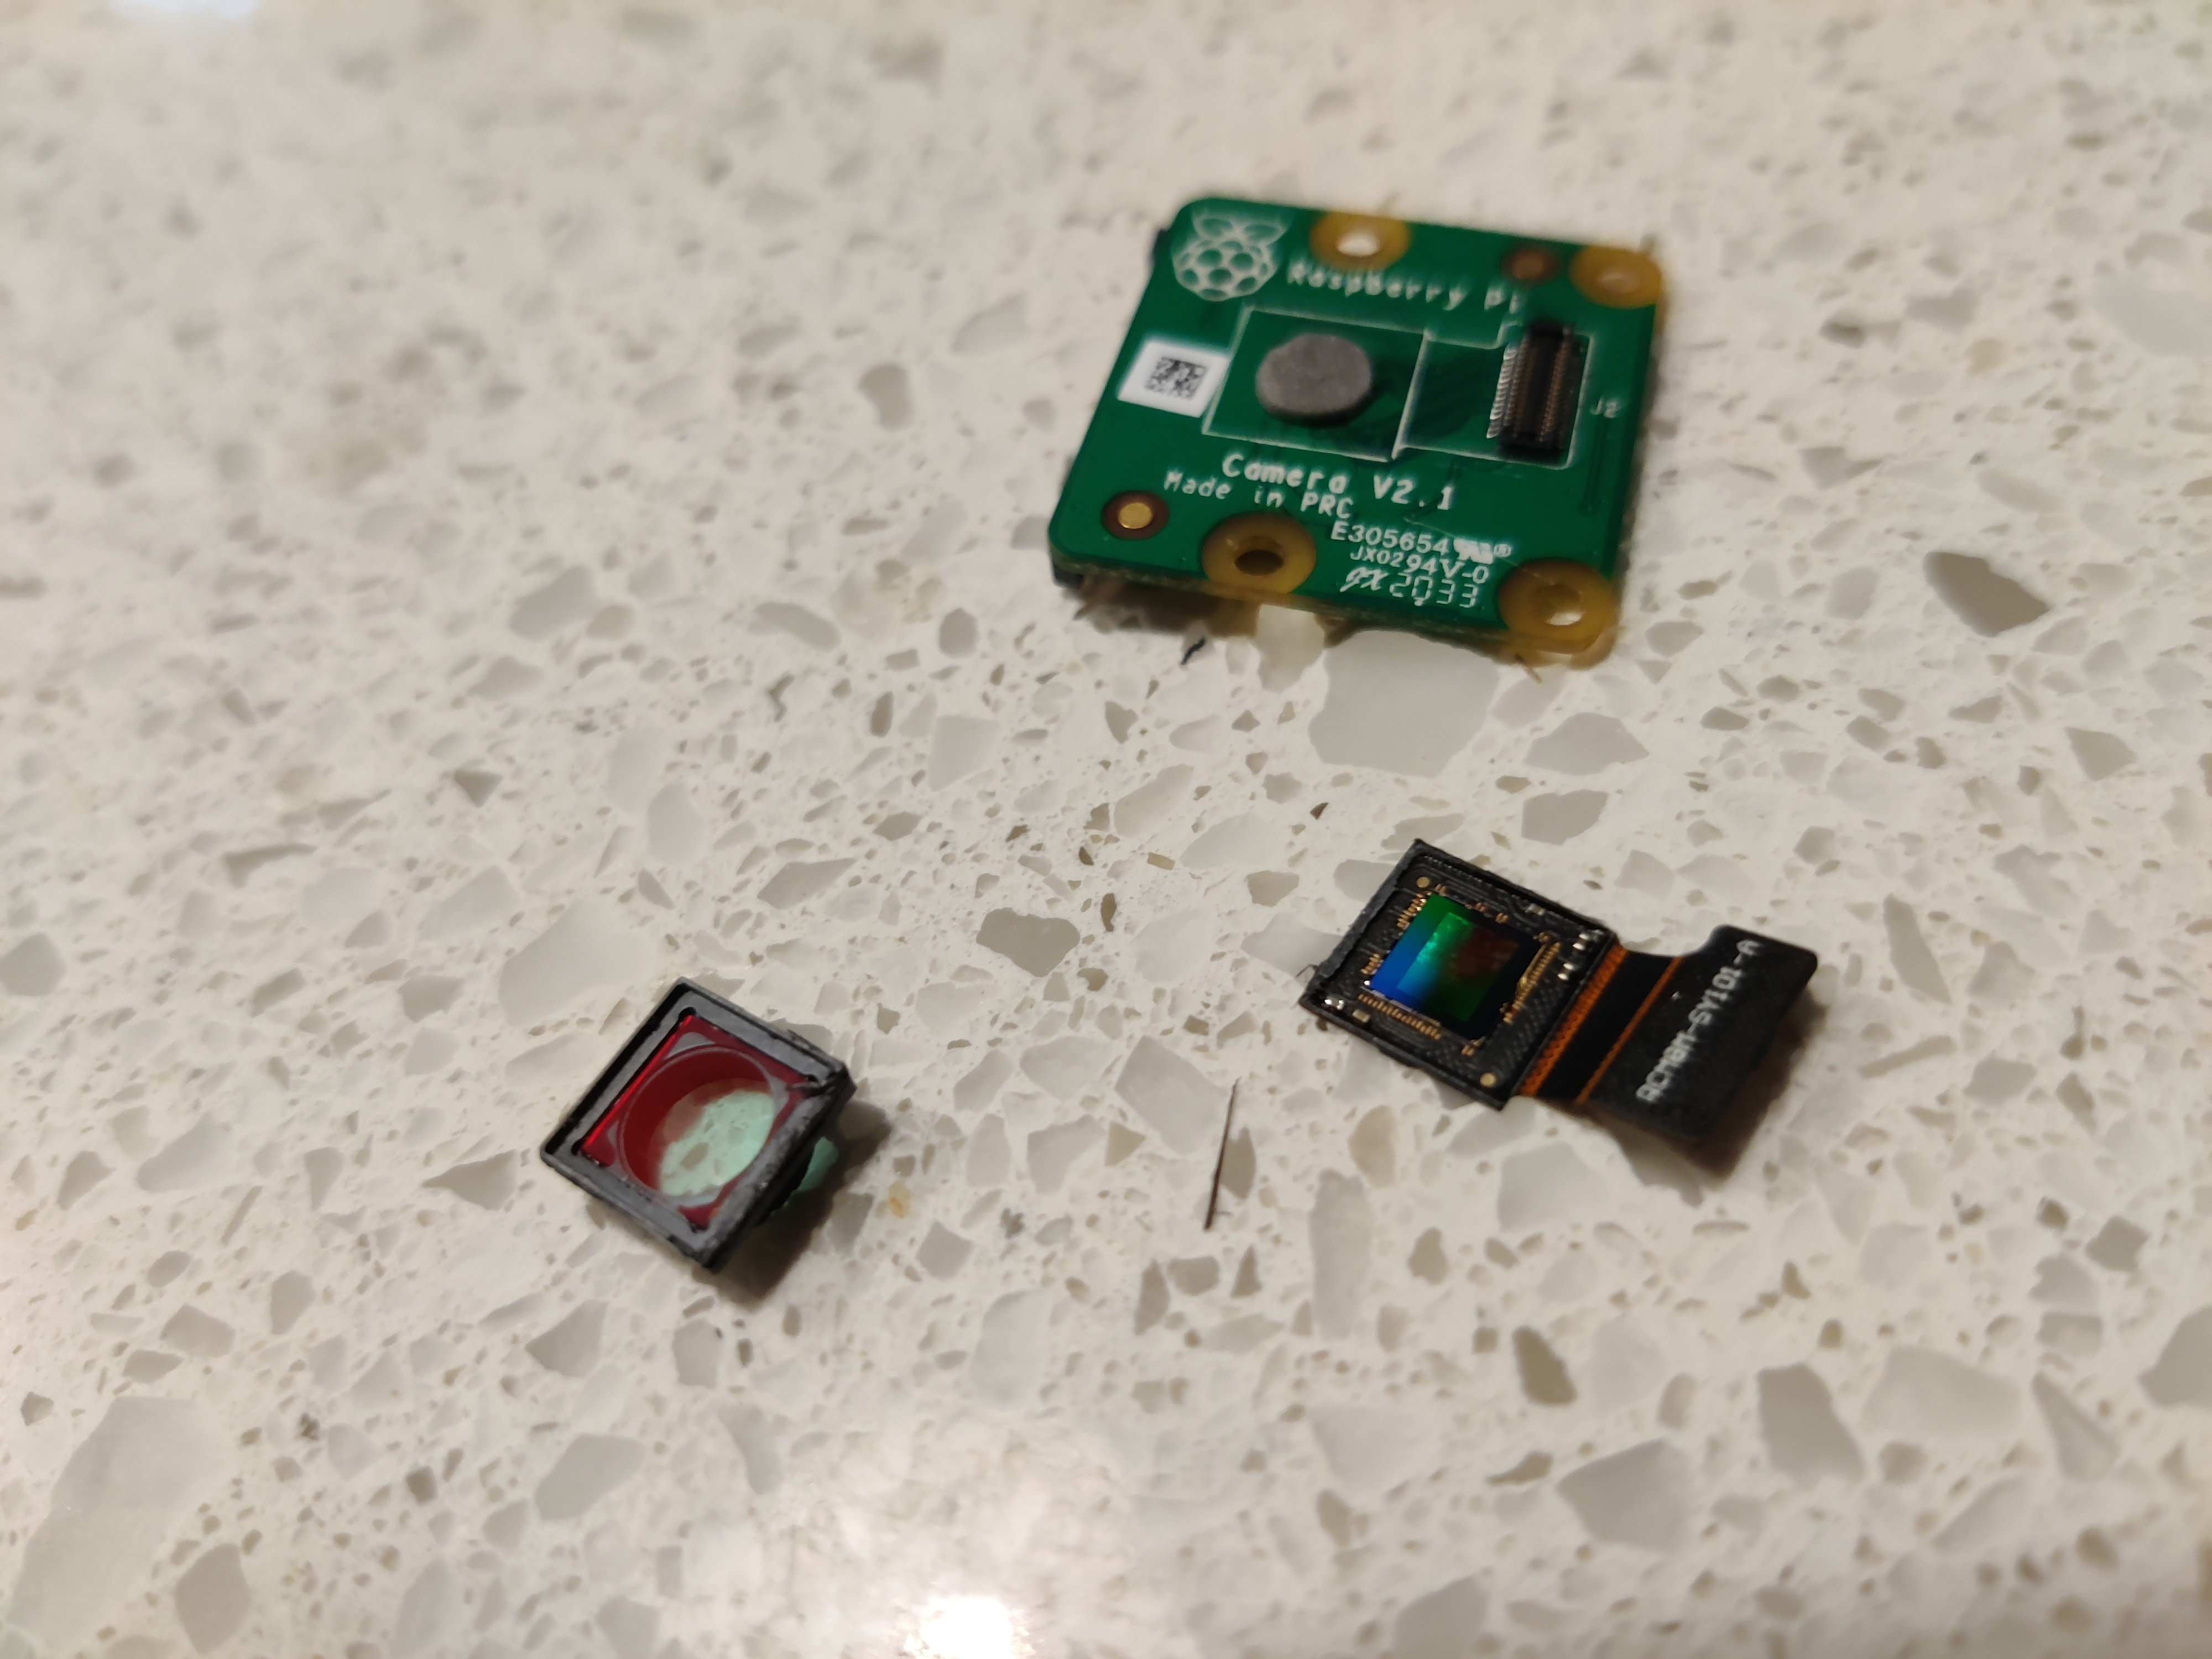
\includegraphics[width=1.0\linewidth]{images/board-filter-sensor}
	\caption{\label{fig:board-filter-sensor}
		The Raspberry PiCam V2 camera board, IR filter, and sensor disassembled to create a DiffuserCam.}
\end{figure}



\section{Results}

\begin{itemize}
	\item I recorded caustics on the sensor by applying 2.5V to the LED and capturing an image for the default exposure time (Fig.~\ref{fig:caustic}).

	\item I computed the autocorrelation of the camera setup's PSF
	      with~\num{2}mm thickness cardboard separating material
	      (Fig.~\ref{fig:psf-autocorrelation-2mm-spacing}).
	      I first normalized the PSF~$X\in\mathbb{R}^{h\times w}$ by
	      subtracting the mean pixel value~$\overline{X}$ and dividing by the standard
	      deviation~$\sigma$ giving
	      \begin{equation}
		      X_{ij} = \frac{X_{ij} - \overline{X}}{\sigma}.
	      \end{equation}
	      The resulting autocorrelation
	      (Fig.~\ref{fig:psf-autocorrelation-2mm-spacing}) resembles a
	      delta function at the center of the PSF, which indicates the
	      suitability of the diffuser and focal length.
	      The autocorrelation of white noise would give a delta function,
	      and so this resemblance shows that the diffuser has a high degree
	      of randomness.
	      For example, if most of the caustic lines in the PSF
	      (Fig.~\ref{fig:caustic}) were parallel to the~$x$-axis, then the
	      autocorrelation would be spread out in the~$x$ direction.
	      Some degree of spread is visible in the autocorrelation image in
	      the~$x$ direction.

	\item Furthermore, the sharp peak of the autocorrelation at the center
	      indicates that the diffuser is in focus at this~\num{2}mm
	      separating distance.

	\item Comparing the autocorrelation cross sections along the~$y$-axis
	      direction
	      (Fig.~\ref{fig:autocorrelation-cross-section-y-axis-2mm-spacing})
	      and the~$x$-axis direction
	      (Fig.~\ref{fig:autocorrelation-cross-section-x-axis-2mm-spacing})
	      further substantiates the observation of PSF spread in the~$x$
	      direction.
	      The peak in the~$y$-axis direction has a spread of only
	      about~\num{50} pixels, while the peak in the~$x$-axis direction
	      has a larger spread of about~\num{150} pixels.
	      The larger spread in the~$x$ direction is also visible directly
	      from the autocorrelation image
	      (Fig~\ref{fig:psf-autocorrelation-2mm-spacing}) as a horizontal
	      smudge.
	      The reason for this increased spread in the~$x$ direction is due
	      to the regularity of the caustic pattern
	      (Fig.~\ref{fig:caustic}).
	      A large proportion of caustics are oriented horizontally.
	      For an evenly distributed autocorrelation spread the caustic
	      orientations would be uniformly distributed.

	\item I recorded an image under the same conditions but this time with
	      an aperture made of black tape on top of the diffuser
	      (Fig.~\ref{fig:caustic-with-aperture}).

	\item I ran gradient descent (GD) reconstruction of a spiral image displayed
	      on my cell phone
	      (Fig.~\ref{fig:gd-spiral-reconstruction-500iters}).
	      I initialized the GD reconstruction with the raw sensor data
	      (Fig.~\ref{fig:raw-data-spiral}).
	      The reconstruction ran for~\num{500} iterations.
	      The update step uses FISTA~\cite{beck2009fast} and a
	      non-negativity projection.
	      GD reconstructed the spiral image clearly after about 200 epochs.

	\item I ran ADMM reconstruction of the same spiral image on my cell phone
	      (Fig.~\ref{fig:admm-spiral-reconstruction-5iters}).
	      ADMM reconstructed the spiral clearly after only one iteration,
	      starting from the raw sensor data.
	      Successive iterations sharpened the spiral image.
	      However, a regular pattern of artifacts in the image outside the
	      spiral became increasingly apparent.
	      These artifacts appeared in the ADMM reconstruction although at a
	      similarly converged point the GD recsontruction
	      (Fig.~\ref{fig:gd-spiral-reconstruction-500iters}) did not show
	      similar artifacts.

	\item Plot reconstruction error over iterations for both GD and ADMM\@.

	\item Reconstructions of illuminated object.
\end{itemize}


\begin{figure}[t]
	\centering
	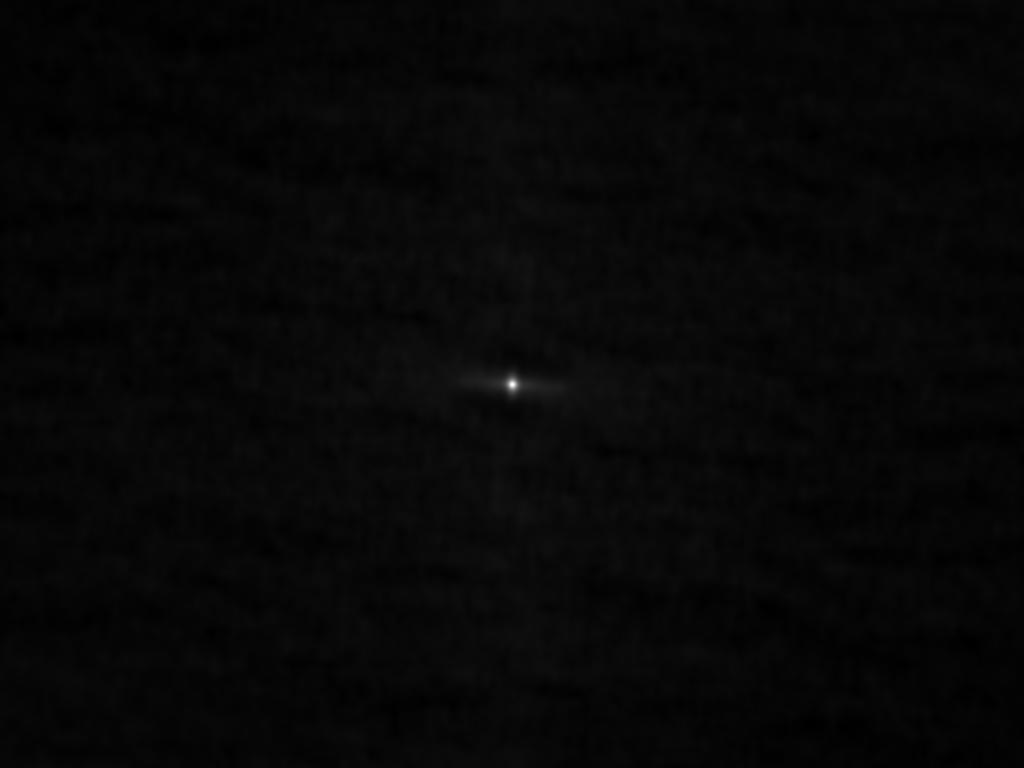
\includegraphics[width=1.0\linewidth]{images/psf-autocorrelation-2mm-spacing}
	\caption{\label{fig:psf-autocorrelation-2mm-spacing}
		Autocorrelation of PSF for camera system setup with~\num{2}mm
		separating material (cardboard).}
\end{figure}


\begin{figure}[t]
	\centering
	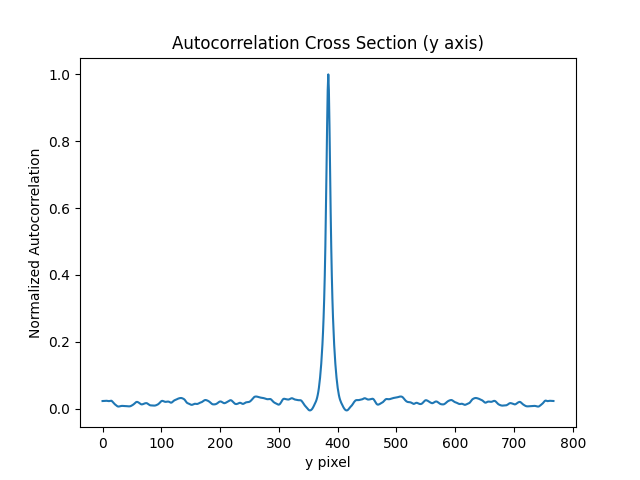
\includegraphics[width=1.0\linewidth]{images/autocorrelation-cross-section-y-axis-2mm-spacing}
	\caption{\label{fig:autocorrelation-cross-section-y-axis-2mm-spacing}
		Cross section of autocorrelation along the~$y$ axis direction.}
\end{figure}


\begin{figure}[t]
	\centering
	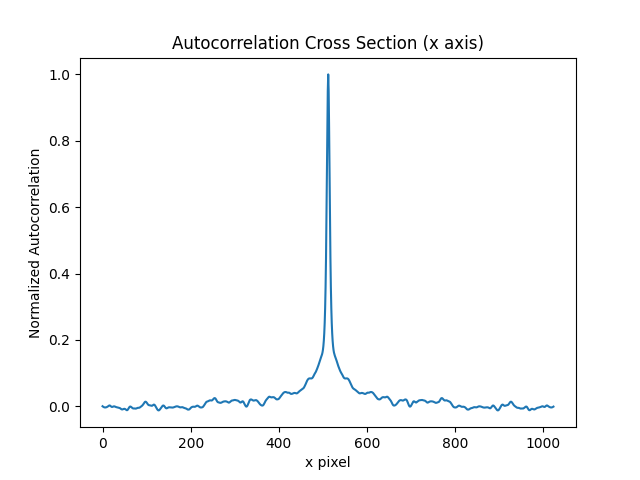
\includegraphics[width=1.0\linewidth]{images/autocorrelation-cross-section-x-axis-2mm-spacing}
	\caption{\label{fig:autocorrelation-cross-section-x-axis-2mm-spacing}
		Cross section of autocorrelation along the~$x$ axis direction.}
\end{figure}


\begin{figure}[t]
	\centering
	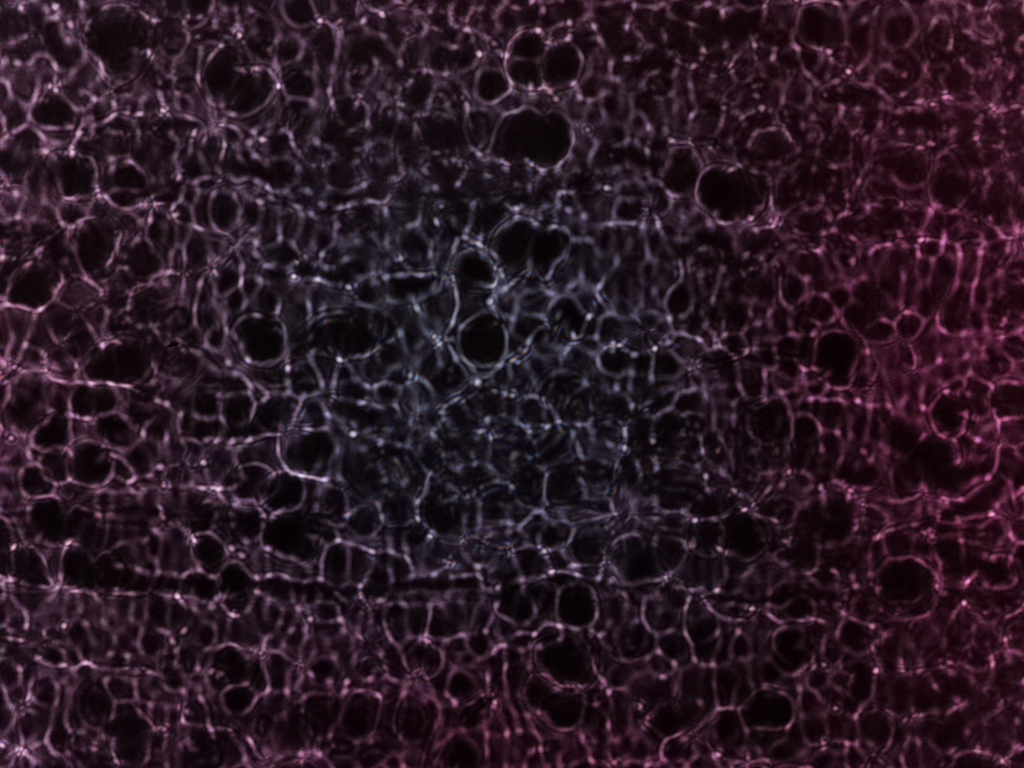
\includegraphics[width=1.0\linewidth]{images/caustic}
	\caption{\label{fig:caustic}
		Caustics produced by applying~\num{2.5}V to the LED\@.
		To form this image the sensor was separated by about~\num{2}mm
		of separating material (cardboard) from the diffuser (double-sided tape).
		Qualitatively, the focal length of the diffuser was about~\num{2}mm.}
\end{figure}


\begin{figure}[t]
	\centering
	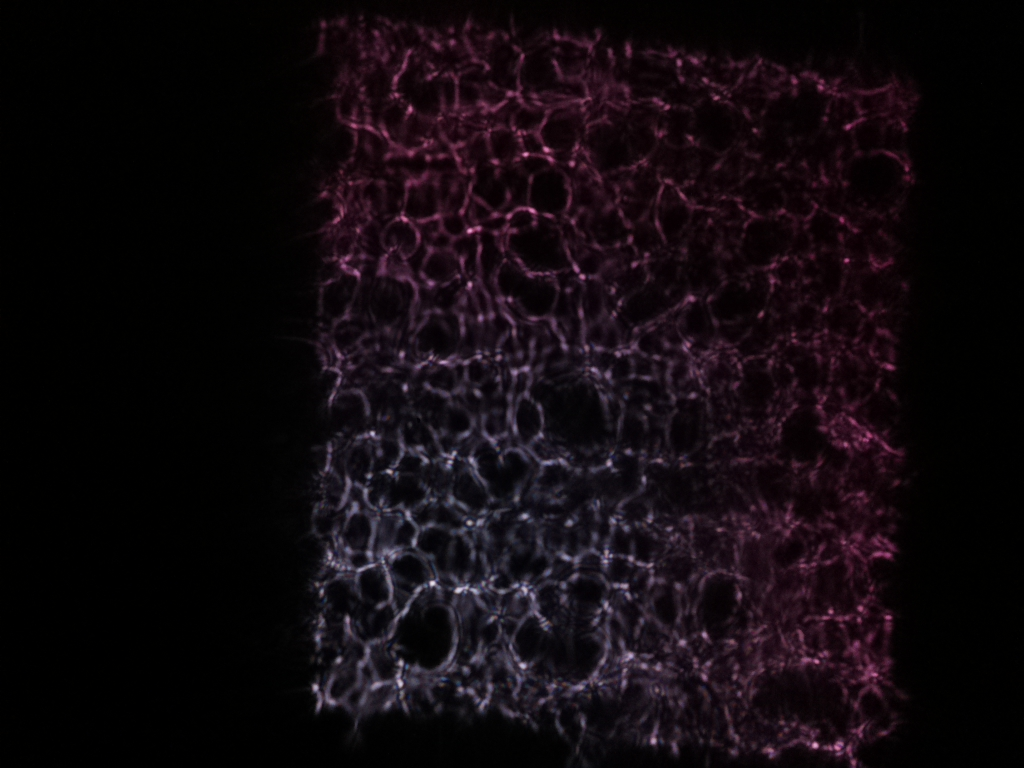
\includegraphics[width=1.0\linewidth]{images/caustic-with-aperture}
	\caption{\label{fig:caustic-with-aperture}
		Caustics produced by applying~\num{2.5}V to the LED\@.
		Here an aperture made from black tape creates a black border
		around the caustic pattern.
		Without the aperture, single-shot calibration would not be
		possible, because new caustics would come into view when the
		point source moves.}
\end{figure}


\begin{figure}[t]
	\centering
	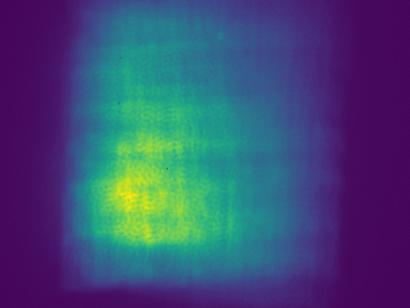
\includegraphics[width=1.0\linewidth]{images/raw-data-spiral}
	\caption{\label{fig:raw-data-spiral}Raw data of the spiral cell phone
		image prior to reconstruction.}
\end{figure}


\begin{figure*}[t]
	\centering
	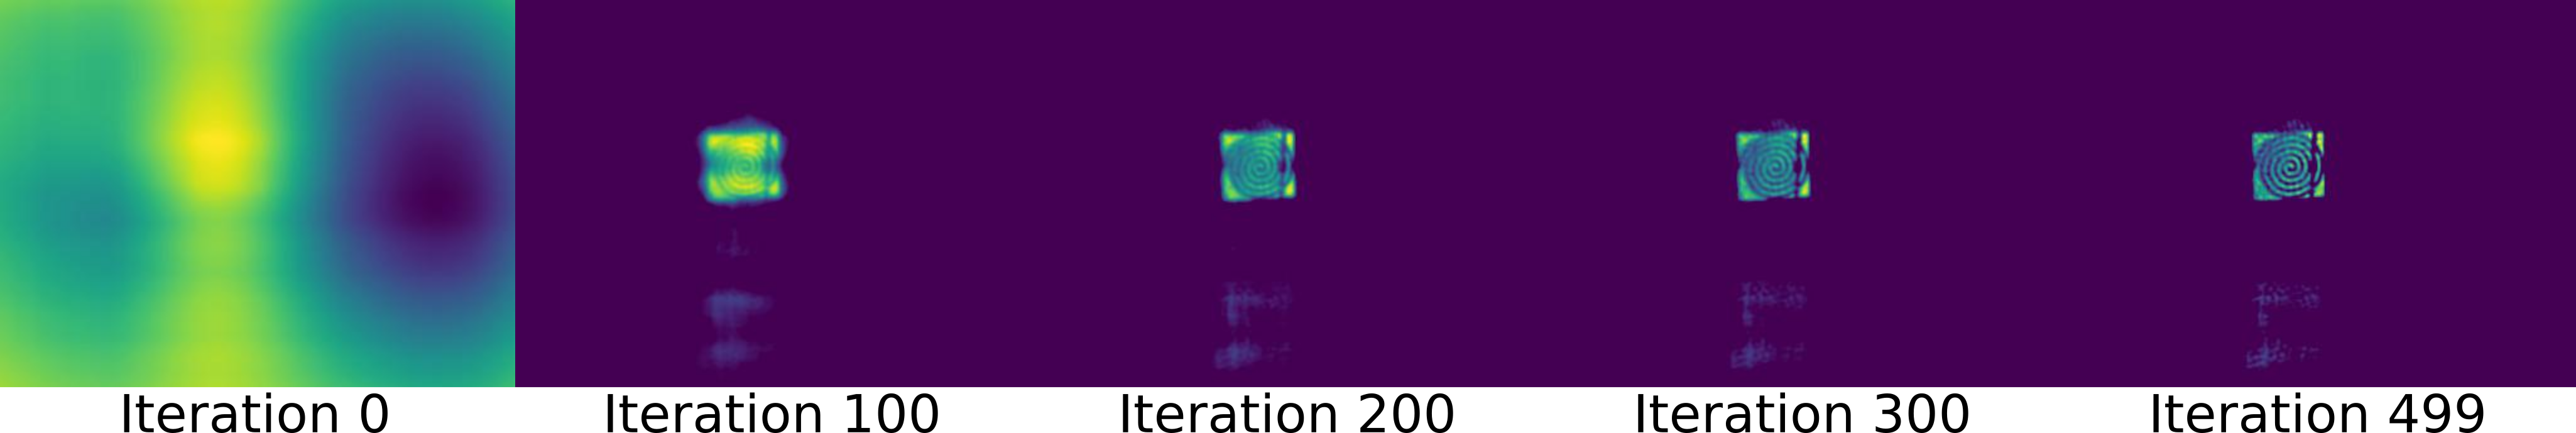
\includegraphics[width=1.0\linewidth]{images/gd-spiral-reconstruction-500iters}
	\caption{\label{fig:gd-spiral-reconstruction-500iters}
		Gradient descent (GD) reconstruction of a spiral image
		displayed on a cell phone in an otherwise dark environment.
		The update step uses FISTA~\cite{beck2009fast} and a
		non-negativity projection.
		GD reconstructs the spiral image clearly after about 200 epochs.
		The bar on the right side of the spiral is an occlusion from a
		stand holding up the cell phone.}
\end{figure*}


\begin{figure*}[t]
	\centering
	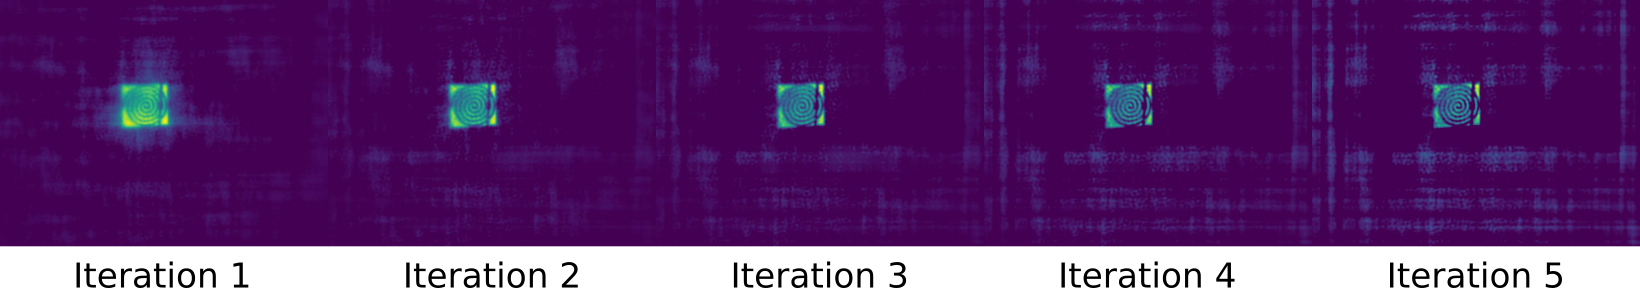
\includegraphics[width=1.0\linewidth]{images/admm-spiral-reconstruction-5iters}
	\caption{\label{fig:admm-spiral-reconstruction-5iters}
		ADMM reconstruction of a spiral image
		displayed on a cell phone in an otherwise dark environment.
		ADMM reconstructs the spiral image clearly after only a single
		iteration.
		The bar on the right side of the spiral is an occlusion from a
		stand holding up the cell phone.}
\end{figure*}



\section{Discussion}

\begin{itemize}
	\item Discussion / analysis about why ADMM produced artifacts and GD
	      did not

	\item Which of ADMM / GD had a lower reconstruction error after
	      convergence?
	      What is the trend?
	      E.g., does GD converge but ADMM diverges?
	      Why?

	\item It was important to analyze the magnification and field of view of
	      the diffuser.
	      Due to the reconstruction step between recording sensor data and
	      viewing an image, it was helpful to find these properties
	      analytically in order to choose appropriate object size and
	      distances to fill the field of view.
	      As with conventional lenses the diffuser's focus distance
	      constitutes a tradeoff between magnification and field of view.
	      The diffuser with a sensor placed distance~$d_i$ from the diffuser
	      magnifies an object placed distance~$d_o$ from the diffuser by
	      magnification~$m = -d_i/d_o$.
	      The size of the cement mixing tray
	      (Fig.~\ref{fig:experimental-setup}) limited the object
	      distance~$d_o$ to a maximum of about~\num{20}cm.
	      Based on qualitative and quantitative
	      (Figs.~\ref{fig:autocorrelation-cross-section-y-axis-2mm-spacing}
	      \& \ref{fig:autocorrelation-cross-section-x-axis-2mm-spacing})
	      observation I used a~\num{2}mm thick cardboard separating
	      material so that the sensor distance~$d_i$ to the diffuser
	      was~\num{0.2}cm.
	      Hence the magnification of the DiffuserCam
	      was
	      \begin{equation}
		      m = -d_i/d_o = -0.01\times,
	      \end{equation}
	      where the negative sign indicates a vertical flip.
	      This magnification affects the size of object imaged at a given
	      focus distance, since the sensor image area is limited
	      to~\num{3.68}mm~$\times$~\num{2.76}mm.
	      Rearranging the magnification in terms of the true object
	      height~$y_o$ and object image height~$y_i$ gives the maximum
	      object height's dependence on magnification, i.e.,
	      \begin{equation}
		      m = -d_i/d_o = -y_i/y_o \implies y_o = -\frac{y_i d_o}{d_i}.
		      \label{eqn:object-height-magnification}
	      \end{equation}
	      Substituting in the known sensor distance~$d_i$, maximum object
	      distance~$d_o$ (determined by the mixing tray's size), and sensor
	      height~$y_i$ gives the maximum object height as
	      \begin{equation}
		      y_o = -\frac{y_i d_o}{d_i}
		      = \frac{0.368\mathrm{cm}\times20\mathrm{cm}}{0.2\mathrm{cm}}
		      = 36.8\mathrm{cm}.
	      \end{equation}
	      In practice this maximum object height was reduced slightly due
	      to the aperture, but served as a rough guideline for the size of
	      object to image in order to fill the field of view.
	      The field of view of the capture setup was large due to the
	      short~\num{2}mm focal length of the diffuser.
	      Increasing to a~\num{4}mm focal length would mean that the camera
	      could only image an~\num{18.4}cm tall object at the same distance.

	\item Analyze the linearity and shift invariance of the system.
\end{itemize}



\par\vfill\par

\clearpage
% ---- Bibliography ----
%
% BibTeX users should specify bibliography style 'splncs04'.
% References will then be sorted and formatted in the correct style.
%
{\small
	\bibliographystyle{ieee_fullname}
	\bibliography{report}
}

\clearpage

\end{document}
